Wireless Sensor Networks (WSN) are widely used in a variety of fields such as healthcare, logistics, military, and environment monitoring. The rapid advancement in Micro-Electro-Mechanical Systems (MEMS) technology has enabled the creation of smart sensors that are significantly more cost-efficient than traditional sensors but are limited in computation, energy and memory \cite{Yick2008, Chai2020, Hussain2021}. These networks can be deployed to provide real-time updates on temperature, humidity, noise and other properties of the environment \cite{Yick2008, Chai2020, Ullo2020}.

Because of their proliferation, environments in which WSNs are deployed are also very diverse, including highly dangerous, inaccessible environments \cite{Prasad2023}. Therefore, the data sent back to the base station can be erroneous, either from hardware, software, communication issues, or any combination of the above. Such erroneous data can lead to incorrect decision-making, wasted resources, and ultimately undermine the reliability of the WSN application. These reasons explain why a robust fault detection system is crucial. Faults in WSN data are typically categorized based on their temporal behavior (time-based) or their impact on sensor readings (characteristic-based). Figure~\ref{fig:types} depicts fault types from both perspective. From a time-based perspective, faults can be classified as soft permanent, intermittent, and transient faults \cite{Prasad2023}. Characteristic-based faults, which describe how the data values themselves are corrupted (e.g., becoming fixed, shifted, or exhibiting other anomalous patterns), also exhibit diverse types according to the literature \cite{Shi2024, Saeed2021, Ni2009, Hasan2024}. The specific characteristic-based fault types considered in this study will be detailed in our fault taxonomy (see Section~\ref{subsec:types}). Understanding these fault types informs the design of the detection algorithms, which we categorize next.

\begin{figure}
  \centering
  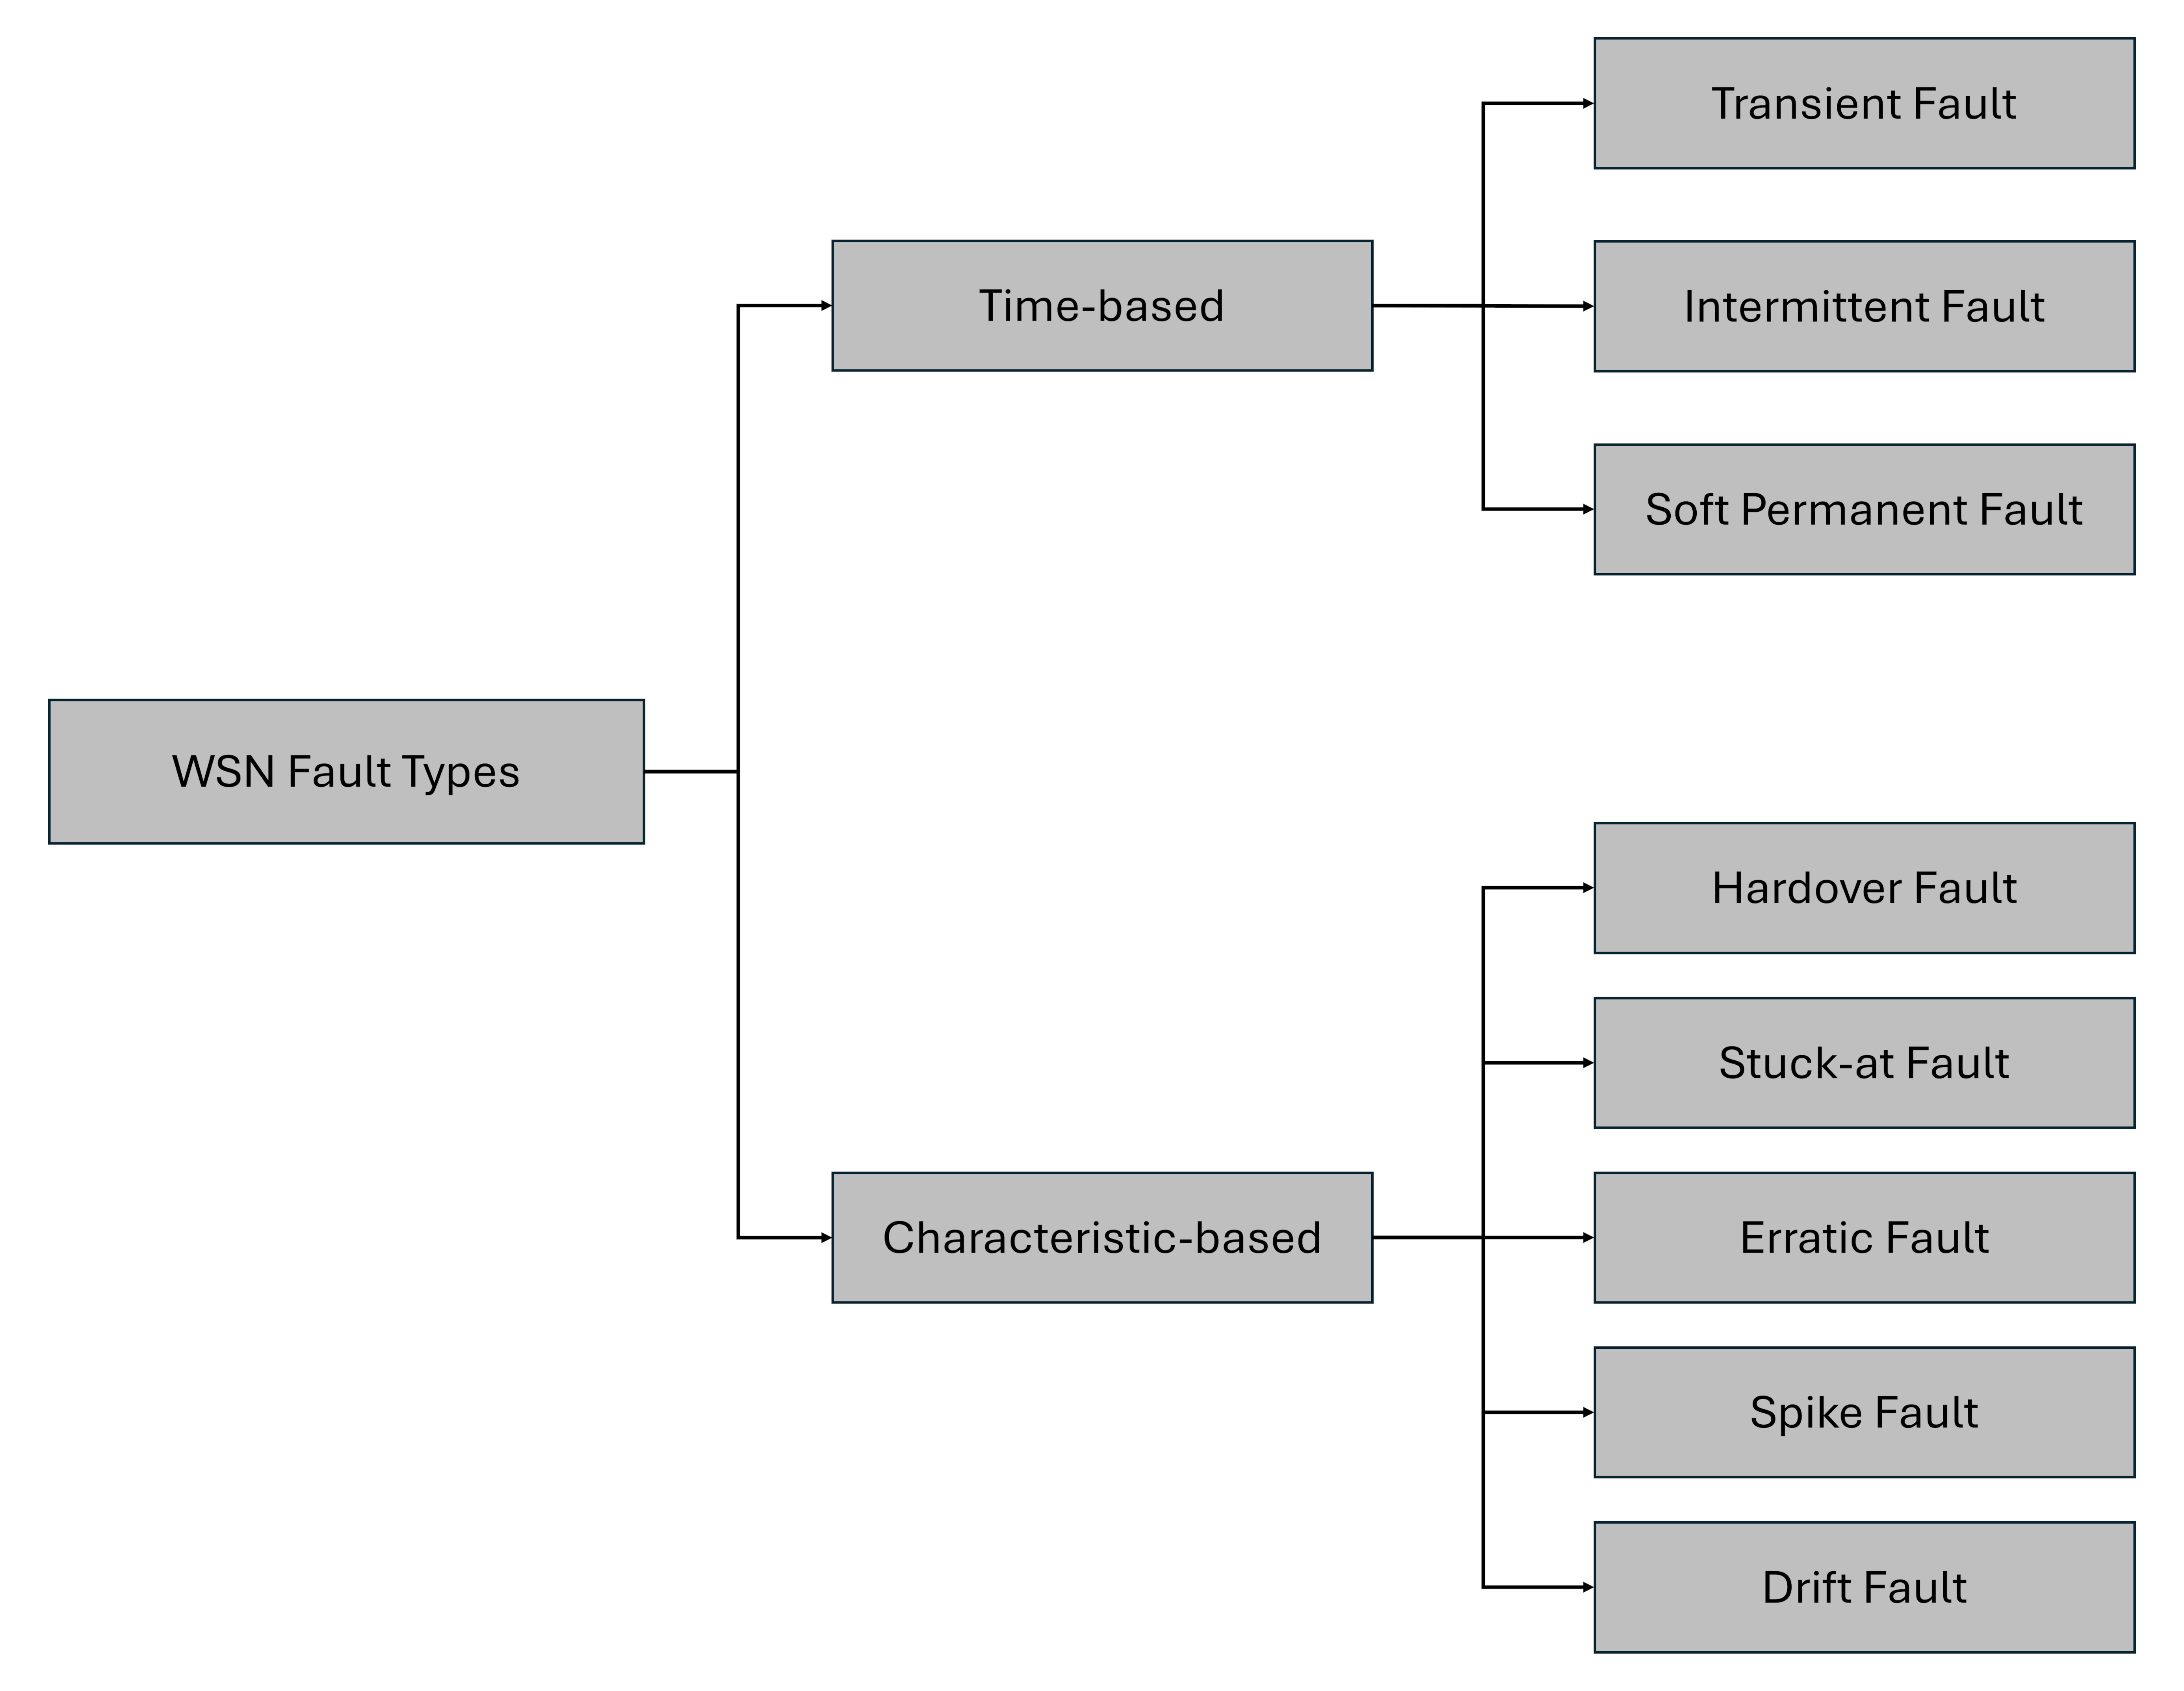
\includegraphics[width=0.8\linewidth]{images/fault_taxonomy.png}
  \caption{WSN Fault Taxonomy}
  \label{fig:types}
\end{figure}

Existing fault detection methods in WSNs include model-based approaches, data-driven approaches and hybrid information-based methods \cite{Shi2024}. The most common approach is a model-based algorithm, which utilize mathematical and statistical principles to model each fault type. The data-driven approach on the other hand uses the analysis of data samples obtained to build a model for fault classification. Hybrid information-based methods use both human knowledge and data through a combination of different methods. Prior work either focuses on temporal patterns at individual nodes or spatial relations across neighbors, but fails to integrate both effectively. Given the complexity of WSN data and the potential for unknown fault patterns, data-driven approaches that can learn from data are particularly promising. Furthermore, a hierarchical architecture can effectively model both local temporal dynamics and broader spatial dependencies. In this work, we investigate the efficacy of a data-driven hierarchical method for WSNs fault diagnosis. The major contribution of this paper are as follows:

\begin{itemize}
  \item Introduce a novel Iterative Graph Network (IGN) that integrates Graph Attention Convolution with a custom Confidence Modulator(CM), dynamically refining node representations through iterative confidence propagation.
  \item Propose HiFiNet, a hierarchical network. HiFiNet first employs a Long Short-Term Memory based stacked autoencoder (LSTM-SAE) at the edge for temporal feature extraction and initial fault screening, followed by IGN for aggregating neighborhood information and refining fault diagnosis.
  \item Create a synthetic WSN dataset using NASA’s MERRA-2 reanalysis data as a substitute for real-world environmental sensor measurements and inject fault to it and Intel Lab Dataset \cite{Intel2004}.
  \item Evaluate performance including various metrics such as: accuracy, F1-score, precision on the aforementioned datasets, demonstrate improvement against methods in the literature.
\end{itemize}
